\documentclass[12pt,a4paper,titlepage,english]{article}
\usepackage[utf8]{inputenc}
\usepackage{amsmath}
\usepackage{amsfonts}
\usepackage{longtable}
\usepackage{amssymb}
\usepackage{graphicx}
\usepackage[a4paper, left=.6in,right=.6in,top=.8in,bottom=.8in,]{geometry}
\usepackage{tabularx,ragged2e,booktabs,caption}
\usepackage{setspace}
\setstretch{1.5}
\usepackage{tabularx, booktabs}

\usepackage{dcolumn} 
\newcolumntype{d}[1]{D{.}{.}{#1}}    
\newcolumntype{Y}{>{\centering\arraybackslash}X}
\usepackage[T1]{fontenc}
\usepackage{babel}
\usepackage{url}


\begin{document}



\title{Cross-checking sources on eighteenth century trade between France and Hamburg\thanks{We are grateful to Ulrich Pfister for sharing data with us and for his comments. This work was funded by the Agence Nationale de la Recherche (Projet TOFLIT18, ANR-13-BSH1-0005)}}
\author{Alexandre Aubourg \thanks{Ministère de l’Économie et des Finances, PARIS, FRANCE}
\and Guillaume Daudin\thanks{
Universit\'{e} Paris-Dauphine, PSL Research University, LEDa, 75016 PARIS, FRANCE \newline
Universit\'{e} Paris-Dauphine, PSL Research University, IRD, LEDa, UMR 225, DIAL, 75016 PARIS, FRANCE \newline
Sciences Po, Observatoire Fran\c{c}ais des Conjonctures \'{E}conomiques (OFCE), 75014 PARIS, FRANCE \newline
email: guillaume.daudin@dauphine.fr}
\and Elisa Tirindelli\thanks{Trinity College, DUBLIN, IRELAND}}




\maketitle

\begin{abstract}
This paper cross checks two eighteenth century trade data sources from Hamburg and France that have been recently digitized.
Both sources respect the Benford's law.
The value of French exports to Hamburg recorded by France is quite different from the value the same exports recorded by Hamburg.
This can be explained by the shortcomings of the two data sources.
Reassuringly, the evolution and composition of trade are well matched.
This suggests that the recently collected sources for eighteenth century trade flows (France, Austrian Netherlands, Britain, Sound...) can be cautiously used to improve our knowledge of the eighteenth century economy.  
\end{abstract}


\section{Introduction}

Much information on past economies may be gained through the systematic collection of trade data.
These are comparatively abundant as foreign trade has long been a sizable source of income for states and the latter have been careful in collecting information on it: series on international trade starting in the eighteenth century exist for several countries and regions such as England, France, Sweden, the Austrian Netherlands, Venice, Portugal, Spain. \cite{charles_eighteenth-century_2015}.
The Sound records go back even further.
This calls for the creation of large databases and there are a number of active projects, under different states of readiness: Ireland, Norway, UK, World \cite{dedinger_exploring_2017}, France \cite{daudin_toflit18_????}, Germany, the Sound \cite{gobel_sound_2010}.
As underlined in \cite{charles_eighteenth-century_2015}, these statistics are only being systematically collected now because of the practical difficulties linked with the raw amount of data that were difficult to solve before IT ressources became much more affordable.
Ancient arguments about the reliability of the data resurface at this occasion.
In France, for example, Bertrand Gille asserted long ago that while external trade statistics are among “the most consistent economic series”, “the numbers produced are often fanciful” and “difficult to match” from one document to another (\cite{gille_les_1964} quoted in  \cite{charles_eighteenth-century_2015}).
These reservations sometime come from the belief that  total value or quantity collection might be more liable to registration errors and fraud compared, for example, to price data collected from \emph{mercuriales}.

Thankfully, the multiplicity of sources allow for cross-checking them by comparing "mirror flows".
The exports from France to Hamburg registered in France are the same trade flow as the imports from France to Hamburg registered in Hamburg.
By comparing these two trade flows, on should be able to determine if the comfort or undermine one another.
One should not expect too much, as it is well known that there are a number of issues with the accuracy of contemporary trade statistics as well \cite{morgenstern_accuracy_1963,rozanski__1994}.
The partner recording methods were not unified  (production or first port of call ?) and are not always well known, the length of the trade voyage may mean that a trade flows is registered in one year by the exporter and the next by the importer, the categorization of goods was not unified before the process that started with the Brussel conference in 1853 \cite{escaith_past_2015}, and the determination of prices, either in the original source or now is fraught with difficulties.
Still it would be encouraging if, despite these difficulties, one where to find commonalities between two different sources.

The digitization of eighteenth century trade data sources for Hamburg and France make cross-checking possible. This is the aim of this paper. It follows similar exercices between French and Sound Toll registers sources \cite{charles_cross-checking_2018} and the sources from Austrian Netherlands that have been recently digitized \cite{charles_comparing_2016}. We have encouraging results.
The distribution of the first digits in both sources respect the Benford's law, which is in favor of the authenticity of the data.
The value of French exports to Hamburg recorded by France is quite different from the value the same exports recorded by Hamburg.
This can be explained by the shortcomings of the two data sources.
Reassuringly, the evolution and composition of trade are well matched.
This suggests that the recently collected sources for eighteenth century trade flows (France, Austrian Netherlands, Britain, Sound...) can be cautiously used to improve our knowledge of the eighteenth century economy.  


\section{Dataset}

This analysis uses to sources of data. The French dataset accounts for exports flows towards all countries whereas for the German dataset only provides imports from France. A quick presentation of each of them is given by \cite{charles_france_2015, weber_hamburg_2015}

\subsection{French Dataset}

\subsubsection{Origin of data}
Data come from the archives of the French \textit{Bureau de la Balance du Commerce}. This institution was created in 1713, after the Treaty of Utrecht, which followed the Spanish succession war. In this circumstances, the French were positively impressed by the detailed knowledge shown by the British on their trade flows and they also decided to create an institution which would keep track of exports and imports from and to France. Before that date, there were already local institutions keeping track of goods going in and out of harbour cities but starting 1716 they started sending their records to the \textit{Bureau}. The \textit{Bureau} would then compute aggregate yearly figures for each \textit{direction} (port) and then send them back to the local chamber of commerce, so that they could correct unit prices or suggest missing ones. A number of these documents survive and form a dataset of French regional trade, but we are not going to look into them closely. On the other hand, another kind of document survived, which reports the total value of trade for each destination for each year, so at least we have reliable figures on aggregate values. Starting from 1750 the \textit{Object Général} was introduced, which was more complete, and was recording each product from and to each destination for all ports. The \textit{Objet Général} survived for many years and this is what I have used for my estimations. For the period preceding 1733, I have estimated the data basing on local sources, as explained in section 3. 

\subsubsection{Figures}
Between 1733 and 1820, the French dataset accounts for 146,963 observations, with incomplete data between 1761 and 1767 and missing data between 1782 and 1787, in 1789 and in 1797. There are overall 82 different destinations recorded, but each one of them is not present every year. Rather then single countries they are groups of countries and most destinations get broken down into smaller destinations in later periods or even disappeared to be replaced by other smaller entities. To bypass this problem I used country grouping. 11 different groups could be created and each of them comprises all the evolution of one destination, so that I can have observations for each group for each year. The groups I am considering are: Germany, England, Flanders and Habsburg Monarchy, Italy, Portugal, Spain, Switzerland, Colonies, Dutch Republic, India, Levant, North. The flows towards Hamburg in particular are 11,062 and data are available for the same period as the rest of of the dataset.\\
Values in the dataset are always expressed in \textit{livres turnois}, but I will convert them in grams of fine silver to be able to compare the French dataset concerning trade towards Hamburg with the German dataset. The value of the \textit{livre} has been constant at 4.505 grams of fine silver all throughout the period in consideration. 



\subsubsection{Limitations of French dataset}
As explained above, data got to us through different sources. The most complete one is the \textit{Objet Géneral} however from 1733 to 1749 it had not been instituted yet and the only available information at product level from the French side are the local sources. Unfortunately, local sources tend to be incomplete and very rarely we still have records from every source and every year, which makes the first part of the dataset quite incomplete. To compensate for this problem I have tried to estimate the data in the first part of the dataset as explained in section three.
In addition to this, another major limitation of the French dataset is that Hamburg does not appear as a destination per se but as part of a broader group denominated “Nord”. Prior to 1733 the destination “Nord” was a general category that included all locations situated north of the Low Countries on the European continent. In 1733 the category “Denmark” was created, that included trade with the actual Denmark and Norway and in 1734 “Suède” was also detached from the “Nord” to form a specific geographical unit (equivalent to our modern Sweden, Finland, and a small piece of land in Western Pomerania). In 1744 “Russie” was further detached from “Nord” and finally in 1780 “Nord” disappeared completely to be replaced by three new geographical entities: “Royaume de Prusse”, “L’Allemagne et la Pologne” and “Les villes Hanséatiques”, the latter including Hamburg, Bremen, Lübeck and Dantzig \cite{charles_cross-checking_2018}.
As a result, in the comparison analysis, we expect the French dataset to report higher figure than what we can find in the Hamburg dataset. 

\subsection{German Dataset}
\cite{pfister_great_2017}
\cite{pfister_quantitative_2015}

\subsubsection{Figures}
The German dataset is unfortunately less complete than the French one, on several points of view. First all of all it comprises of only 1609 observations and it covers the following years: 1736-1740, 1742, 1747, 1753, 1755, 1756, 1760, 1762, 1763, 1769, 1770, 1771, 1773, 1776, 1781-92, 1794, 1795, 1797 and 1798. The flows recorded however are not as detailed as in the French dataset. In this case we find broader categories of products, which correspond to several goods in the French dataset. We count 39 categories, to which we add a fortieth one that includes all the French goods that cannot be classified in the Hamburg categories. 
%\newpage
\begin{center}
\captionof{table}{Classification Hamburg} \label{tab:title} 
\begin{tabularx}{1\textwidth}{|c *{5}{|Y}|}
\hline
	Eau de vie & Saffron & Tar & Turpentine & Cacao \\ \hline
	Tobacco & Spermaceti & Indigo & Verdigris & Coffee \\ \hline
	Wine & Olive Oil & Minium  & Vitriol & Ginger \\ \hline
	Pernambouc Wood & Tallow & Lead Oxyde & Candles & Pepper \\ \hline
	Painting Wood & Whale Oil & Potassium & Butter & Sugar \\ \hline
	Cotton & Alun & Soap & Fruits & Tea \\ \hline
	Gum & Cochineal & Sumac & Rice & Iron \\ \hline
	Lead & Gal & Potassium Bitartre & Vinegar & \  \\ \hline
\end{tabularx}\\~\\
\end{center}

Values are expressed in \textit{Mark Banco}, which, on the contrary of \textit{livre tourois}, was not constant in terms of grams of silver over the period of analysis. For this reason, I had to use a different conversion value for each year. In general however, \textit{Mark Banco} was on average worth twice as much as French \textit{livres}. A table of conversion for \textit{Mark Banco} can be found in the appendix. \\



\subsubsection{Limitations}
As mentioned before, the data come from the Hamburg import toll register, so all taxable goods were recorded in the data. However there were some exemptions for taxes so that some goods were not registered. According to Pfister (2015), only goods coming into the city were liable to paying tolls, coal and grain were exempted and most of dyestuff was not being tracked either. In addition to this, there is the issue of categories rather than products. Unfortunately only a minor share of products can be matched, but on the other hand they represent a vary high share in value terms. 

\subsection{Estimation of French missing data}
As mentioned above, for the whole period preceding 1749, the only available data we have from the French source is either the yearly aggregate figures by destination, or the incomplete local sources, which on the other hand contains information on each product. For this reason, in order to perform the comparison between the two datasets and the subsequent analysis, it will be necessary to estimate the full value of exports from the available data. In order to do this, I run the following regression:
\begin{center}
$\ln(product_{i,j,k,t})=\beta_0 + \beta_1year_t+\beta_3direction_k$
\end{center}
where the dependent variable products stands for the value of exports of one product, for each port reported in the local source and for each year. Year is a set of year dummies and direction is also a set of dummies that indicates in which port the data were recorded (direction also includes “France”, meaning all ports). This model aims to predict the export value of single products per year basing on the yearly changes in export and on the export composition by source, with the assumption that the composition is constant through time. I run the model on the whole available data including those recorded after 1789 and before 1733 but I only do so for coffee, sugar, wine, eau vie and an aggregate category of all other goods (other), except in the case of Hamburg for which I was able to estimate the value of all products. In addition, to avoid the problem of log of zero trade flows, I have substituted them with 0.001, so that observations would not drop but the zero flows in the estimation could be taken into account as a value really close to zero. Finally, I also added weights on value, as to give more importance to flows higher in value. The results are pretty satisfactory; the correlation is very close to 1 for most goods and the pattern of estimated and actual value are very similar. 

\subsection{Testing Benford’s law}
As a last step in my validation of the data, I have tested Benford’s law or the first-digit law on both datasets. Benford’s law is a law providing the frequency distribution of the first digit in most real life datasets. According to Benford the leading digit $d$, with $d \in \{1,...,9\}$ should follow the probability distribution: 
\begin{center}
$P(d)=\log_b(1+\frac{1}{d})$
\end{center}
where $P(d)$ is proportional to the distance between $d$ and $d+1$ on a logarithmic scale, which is the case when the logarithm of the numbers and not the numbers themselves are uniformly and randomly distributed. I run the following Pearsons’s chi square test:
\begin{center}
$$\chi^2=N\sum_{d=1}^{9}\frac{(p(d)-d(b))^2}{d(b)}$$
\end{center}
where N is the frequency and $p(d)$ and $d(b)$ are the proportions of Benford’s law and my data respectively. For both dataset I cannot reject the null hypothesis that the leading digit is actually distributed according to Benford’s law.


\begin{center}
\captionof{figure}{Benford's law}
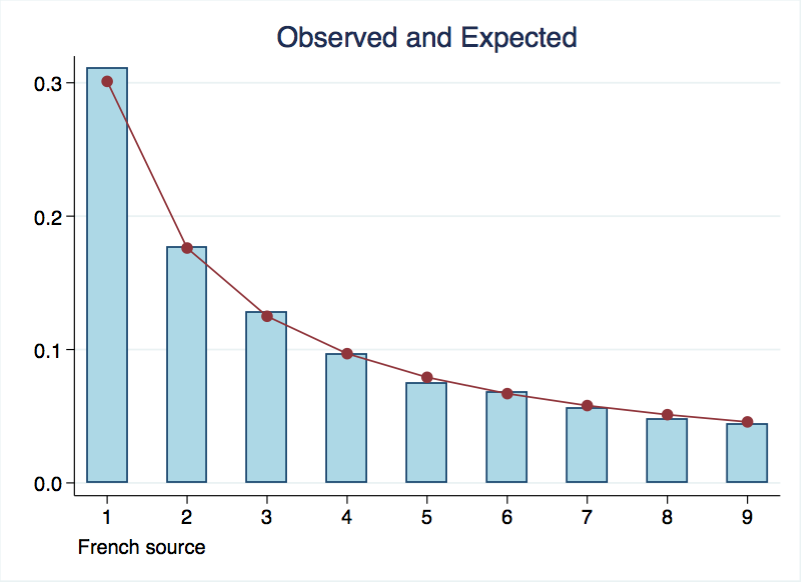
\includegraphics[scale=.28]{benford_fr.png}
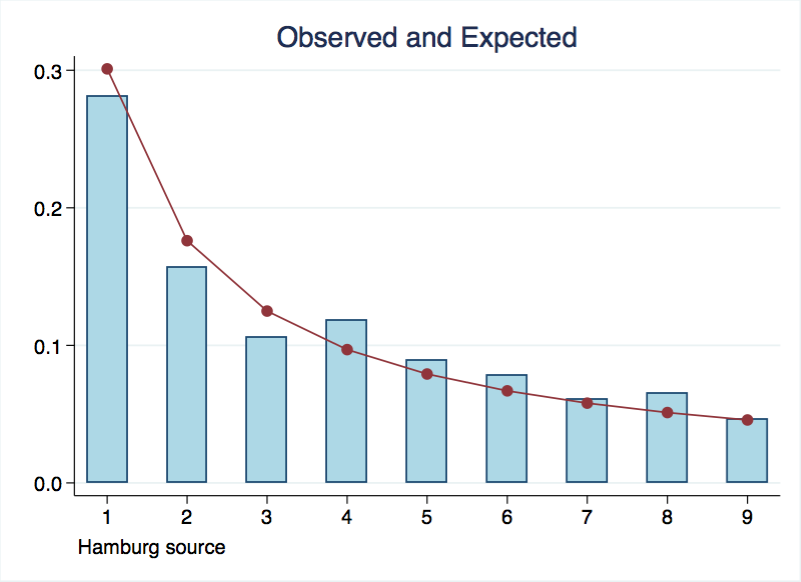
\includegraphics[scale=.28]{benford_hb.png}
\end{center}



\section{Reliability of dataset}
\subsection{Method}
As mention before, an important step of my work is to ensure the reliability of the data. In order to do so I have looked at three different aspects of comparison: the composition of exports by products, by sector and total exports. For the comparison by product I will use the categories present in the Hamburg dataset and compare goods in the French dataset that can be classified within those categories. As per the comparison by sector, I will use the Standard International Trade Classification (SITC revue 3), which is a classification maintained by United Nations and used to compare trade flows across countries and across years. It is based on the materials used in production, the processing stage, its use, its importance in terms on world trade and finally its technological changes.  A table with the category is displayed below. Details of classification of goods into SITC can be found in the appendix.

\captionof{table}{SITC Rev. 3} \label{tab:title} 
\begin{center}
\begin{tabular}{ | l | l | l | l | }
\hline
	0a & European foodstuff and live animals & 6e & Wool products \\ \hline
	0b & Extra-European foodstuff & 6f & Silk products \\ \hline
	1 & Drinks and tobacco & 6g & Coton products \\ \hline
	2 & Crude materials, inedible, except fuels & 6h & Other mixed cloths \\ \hline
	3 & Fuels & 6i & Other mixed textiles \\ \hline
	4 & Oils & 6j & Metal products \\ \hline
	5 & Chemical products & 6k & Other industrial product by composition \\ \hline
	6a & Leather products & 7 & Machines and transport \\ \hline
	6b & Wood products & 8 & Various manufactures \\ \hline
	6c & Paper products & 9a & Precious metals \\ \hline
	6d & Linen products & 9b & Mixed flows \\ \hline
\end{tabular}\\~\\
\end{center}

The composition of exports by products and sector can be analysed both as an aggregate over the available years or in their evolution in time (i.e. looking at total export per year of each products and its evolution). Total exports of course can only be looked at in their longitudinal evolution. In addition, since in some years we have the value from one source but we do not have the value from the other, all comparison can be done either on all the whole period or only on years common to both datasets. As a general results in the analyses we do not see a major difference between results from the latter two cases, which leads us to conclude that common years are a good proxy for the entire period. 

\subsection{Classified versus non classified products}
As a first step, I will look at the ratio of the products that can be classified to those that find no match in the other dataset. As mentioned before, it was necessary to regroup French goods into Hamburg categories to make comparison possible. This results in the matching of 1,913 French goods out of 4,695. At first sight this might be a discouraging result, however if we now look at the share of value of classified goods to total, according to both sources we can see that they actually represent 96\% of the total export. This result holds both if we consider only common years (i.e. excluding years for which only one source is available) and the whole period. \\
The share of not classified goods however varies over the period. As mentioned above, the average is around 4\%, however for most of the period it is below this level. This is compensated by three peaks in 1733 to 1739, 1757 to 1663 and 1780 to 1781 (the latter on a smaller scale), which coincide with the major conflict that occurred in that period. I will analyse the impact of conflict on trade flows more in details in sections 5 and 6.

\subsection{Absolute value of exports from the two sources}
Despite the fact that classified and not classified goods are very close in their share according to both dataset, there is a problem arising while considering the absolute value of export. Since the geographical scope of the two datasets is considerably different at least until 1780, we expect France to overestimate exports, which is exactly what the graph below suggests.
\begin{figure}
\captionof{figure}{Sum of total export according to the two sources}
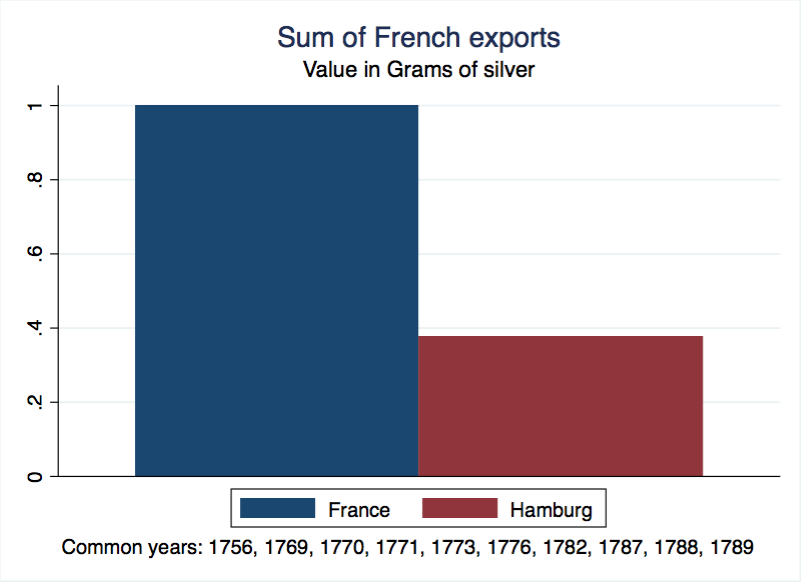
\includegraphics[scale=.28]{value_total_fr_hb_commonyears.png}
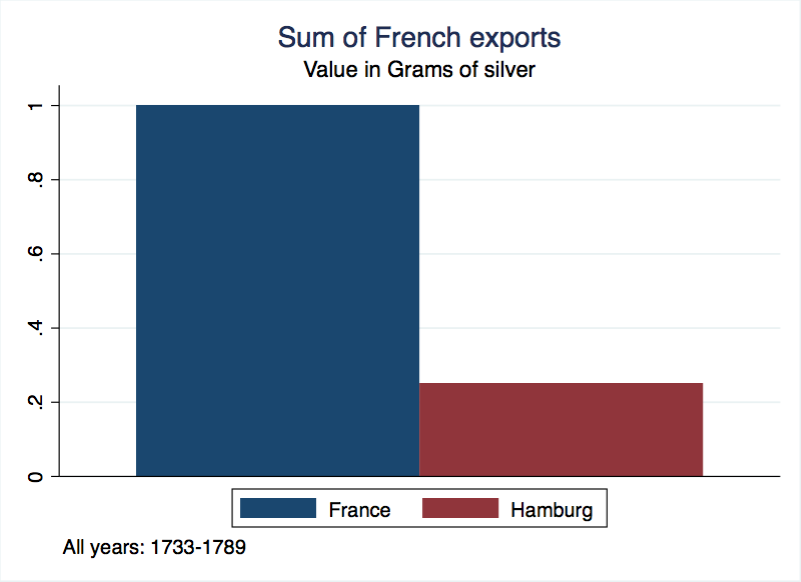
\includegraphics[scale=.28]{value_total_fr_hb.png}
\end{figure}
Aggregate exports value in Hamburg source account for slightly less then 50\% of export value in the French source considering only common years and slightly around 30\% considering all years (1733-1789). The ratio of the two values however is far from stable; before 1740, the two sources report roughly the same value, Hamburg reports even more than France in 1735, which however might be due to the fact that the values I estimated for the period previous to 1753 for France are underestimating the real total value of exports. In the subsequent period there is a sharp decrease, and the ratio stabilizes around 5\%. Surprisingly, no major effect is evident in 1740 with the exclusion of Russia and in 1780, with the narrowing of the destination on the French dataset from “Nord” to “Hanseatic cities”. On the contrary, the ratio increases. This leads me to think either to a mistake in the data, or that the share meant for Russia was only a small part of the overall export towards North.

\begin{center}
\captionof{figure}{Evolution of the ratio of datasets}
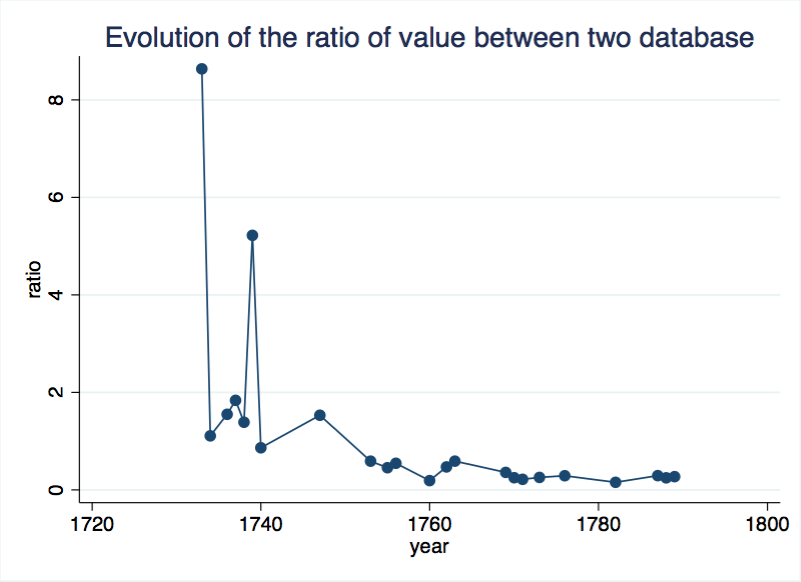
\includegraphics[scale=.3]{long_ratio.png}
\end{center}


\subsection{Comparison of total exports}
I will now turn to the evolution of aggregate exports per year.  For simplicity in comparison I have used value indexed at values in year 1787, which is the most complete for both sources. In this way I can observe better  the pattern of the two series, without considering the discrepancy in absolute value. 
From the graph below it is evident that the two sources move quite well together, with a correlation between the two series of 0.88. Also the data preceding 1740, which are an estimate, are in line with the Hamburg series. 
The overall trend of both series looks like an increasing one even though the growth is interrupted during war period. The Polish succession war between 1733 and 1738, did not seem to impact trade as much as colonial wars, whose effect on the other hand is very evident in the sharp decrease in 1761 and 1781. In this respect, I will go more into details in subsequent sections.

\begin{figure}
\centering
\caption{Comparison of longitudinal evolution of aggregate exports}
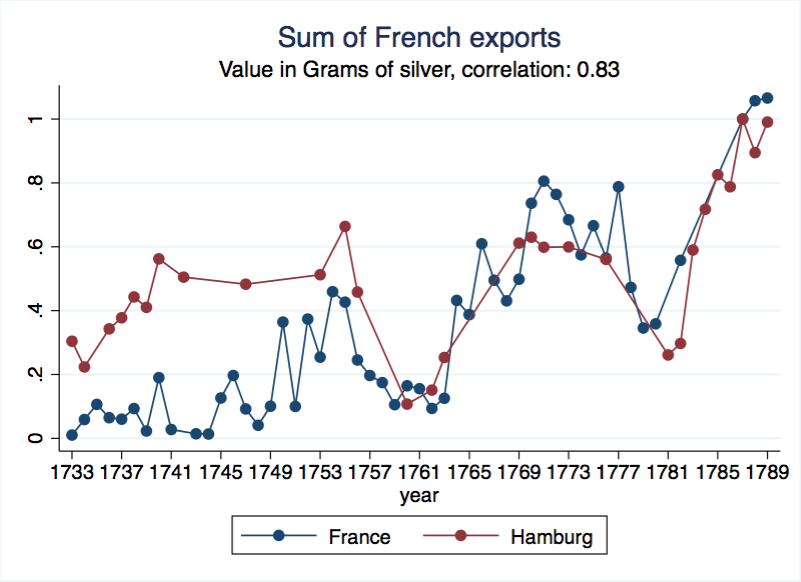
\includegraphics[scale=.3]{long_evolution.png}\\~\\
\end{figure}

\subsection{Comparison at sector level}
\subsubsection{Comparison of aggregate export by sector}
The comparison at sector level brings contrasting results. At aggregate level the two sources are very close, both for the whole period and common years. It is evident that the major sector is exotic foodstuff, followed by beverages and tobacco and then by raw material, which however represents a significantly smaller share. Colonial imports are actually representing the biggest source of trade, which explains why then colonial wars were the cause of trade collapse. \\~\\
\captionof{figure}{Comparison of total exports}
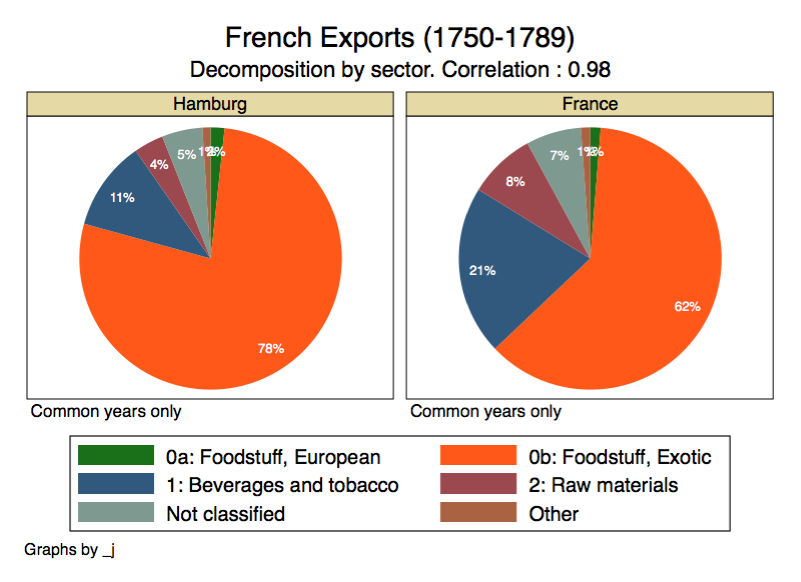
\includegraphics[scale=.28]{commonyears_sector.png}
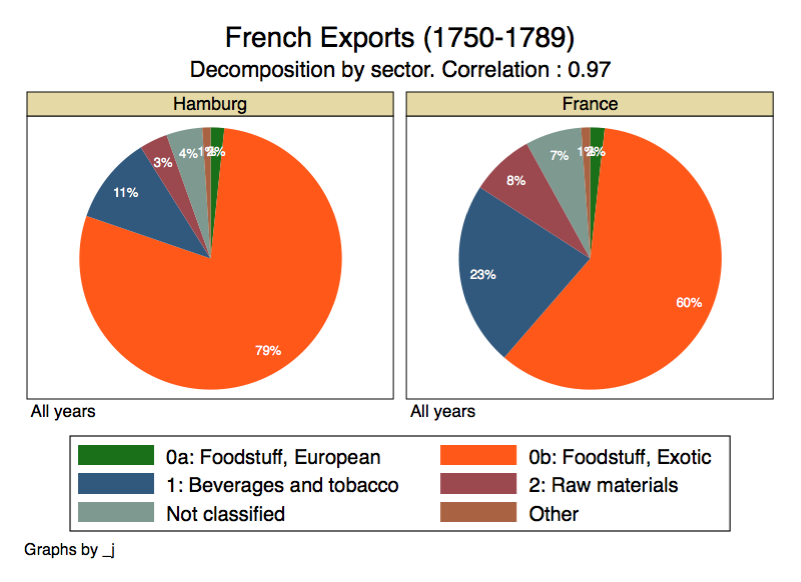
\includegraphics[scale=.28]{allyears_sector.png}

\subsubsection{Comparison of the evolution of major sectors overtime}
As mentioned above the three major sectors are Exotic foodstuffs, beverages and tobacco and raw material, with a higher importance given to the first two. The tables below plot the longitudinal evolution of these sectors according to the two different sources. Results are not as satisfactory as in the total exports longitudinal evolution above and it might be the case the estimation on the values of product pre-1750 was not too accurate because of lack of data. In all the three cases displayed below, I plotted both the share of the sector on the total and the absolute value (indexed at the 1787 value). 
\captionof{figure}{Evolution of Exotic foodstuff}
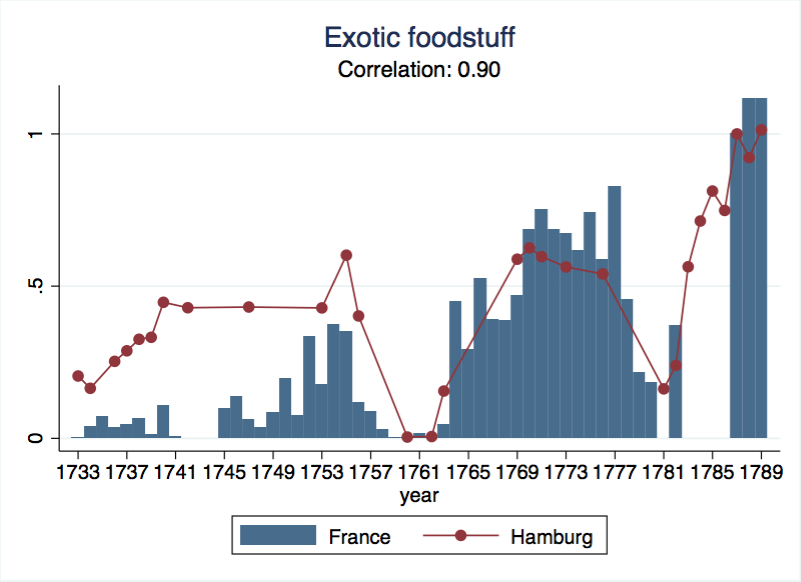
\includegraphics[scale=.28]{exotic_food_long.png}
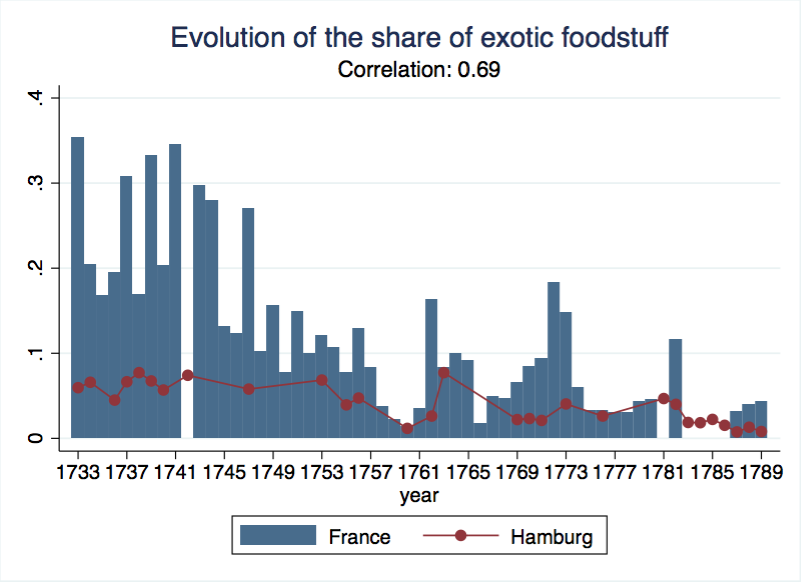
\includegraphics[scale=.28]{exotic_food_share.png}\\
\caption{Evolution of Beverages and Tobacco}
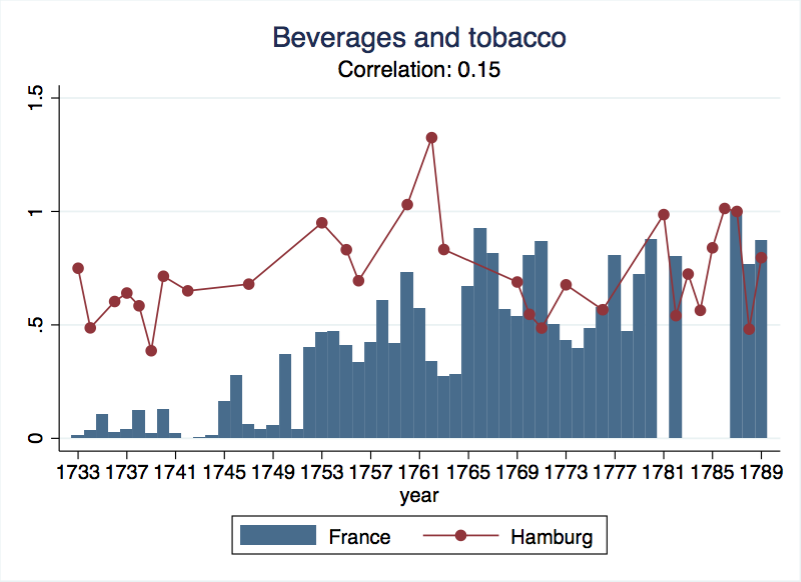
\includegraphics[scale=.28]{bev_tobacco_long.png}
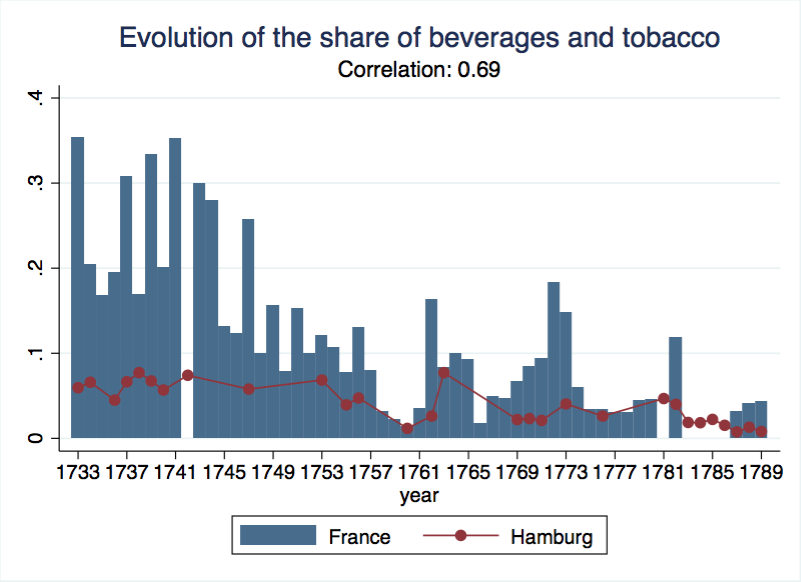
\includegraphics[scale=.28]{bev_tobacco_share.png}\\
\newpage
\caption{Evolution of Raw material}
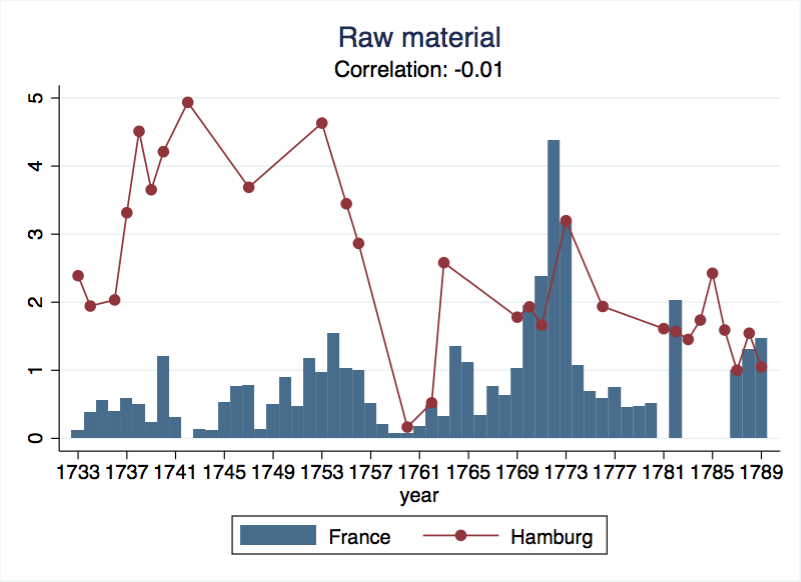
\includegraphics[scale=.28]{raw_mat_long.png}
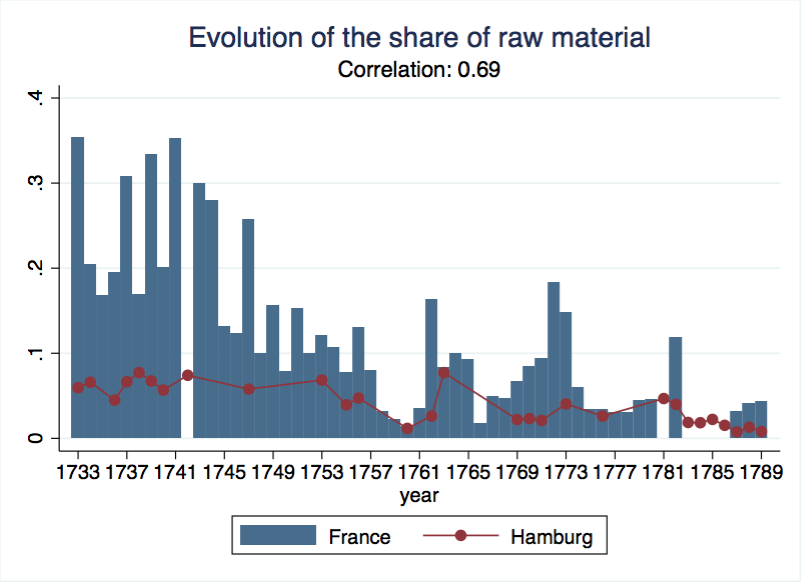
\includegraphics[scale=.28]{rawmat_share.png}

\subsection{Comparison at product}
\subsubsection{Comparison of aggregate export by product}
As for the case of sectors, products do not always give the results we would expect. At aggregate level both on all years and common years the two databases are quite close:\\~\\
\captionof{figure}{Evolution of coffee}
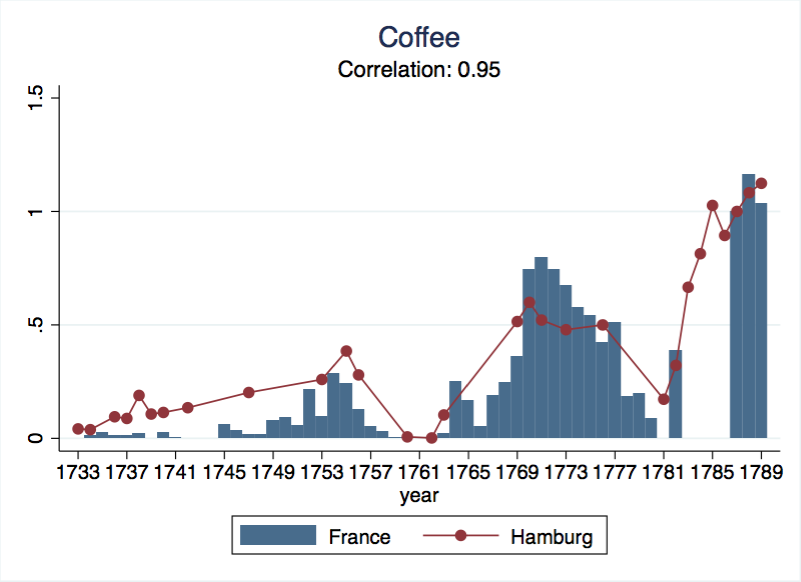
\includegraphics[scale=.28]{coffee_long.png}
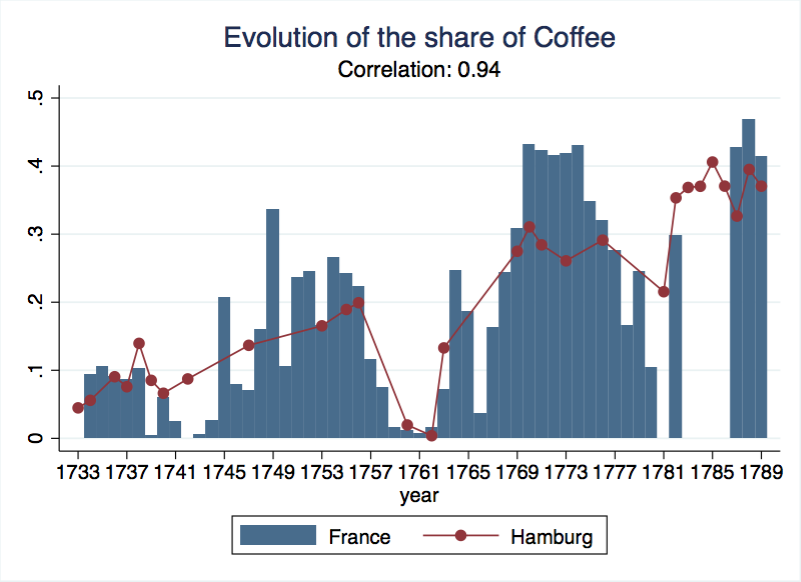
\includegraphics[scale=.28]{coffee_share_long.png}\\
\newpage
\captionof{figure}{Evolution of Sugar}
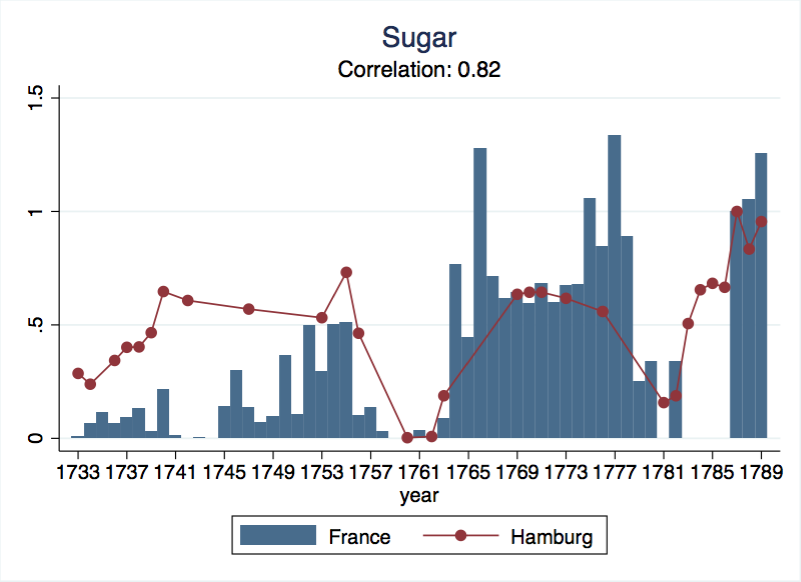
\includegraphics[scale=.28]{sugar_long.png}
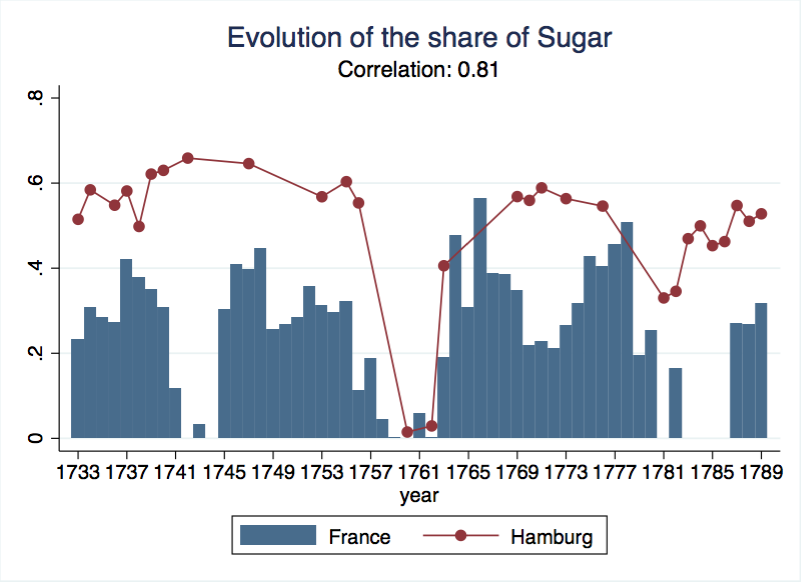
\includegraphics[scale=.28]{sugar_share_long.png}\\
\captionof{figure}{Evolution of Indigo}
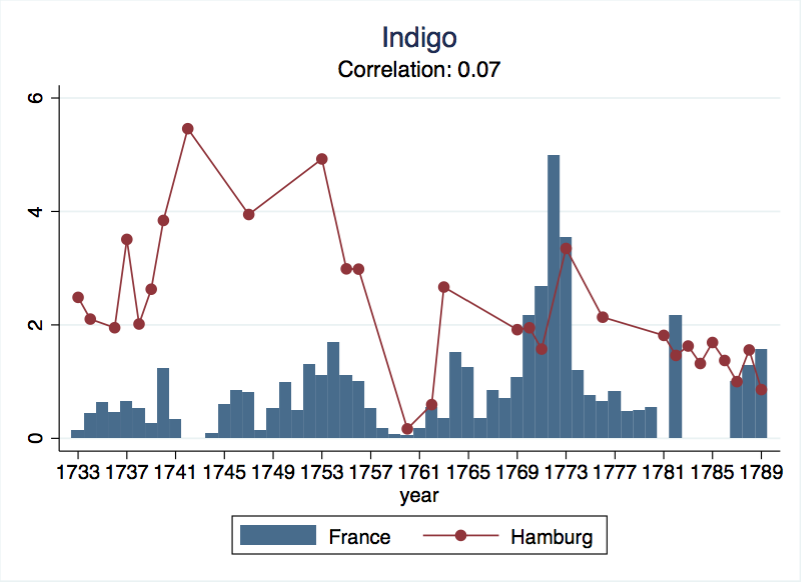
\includegraphics[scale=.28]{indigo_long.png}
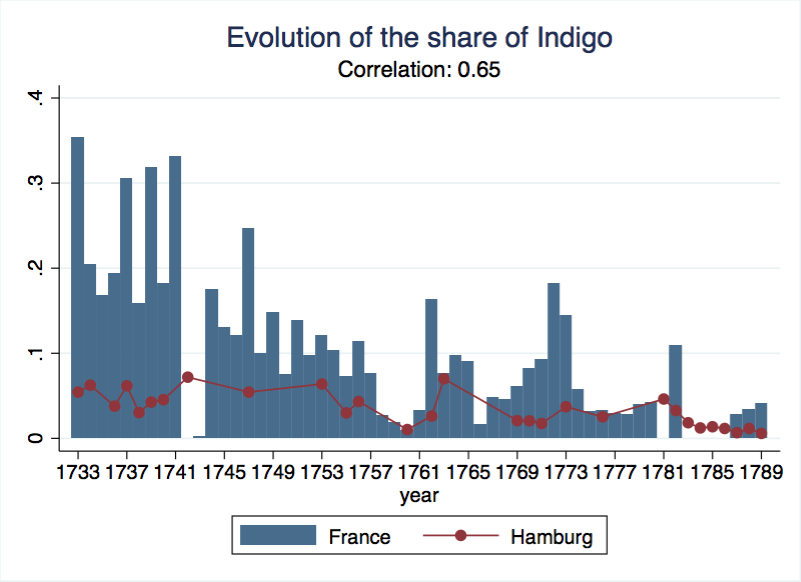
\includegraphics[scale=.28]{indigo_share_long.png}\\
\captionof{figure}{Evolution of Eau de vie}
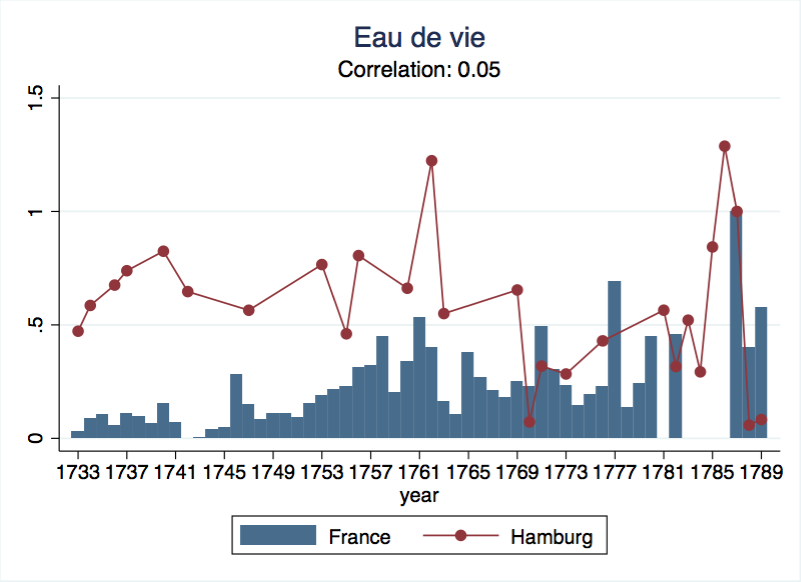
\includegraphics[scale=.28]{eaudevie_long.png}
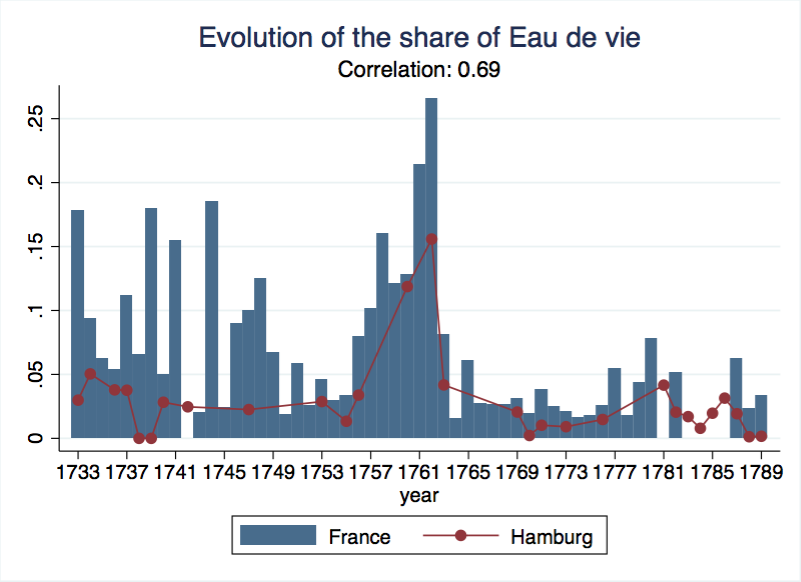
\includegraphics[scale=.28]{eaudevie_share_long.png}\\
\begin{figure}
\caption{Evolution of wine}
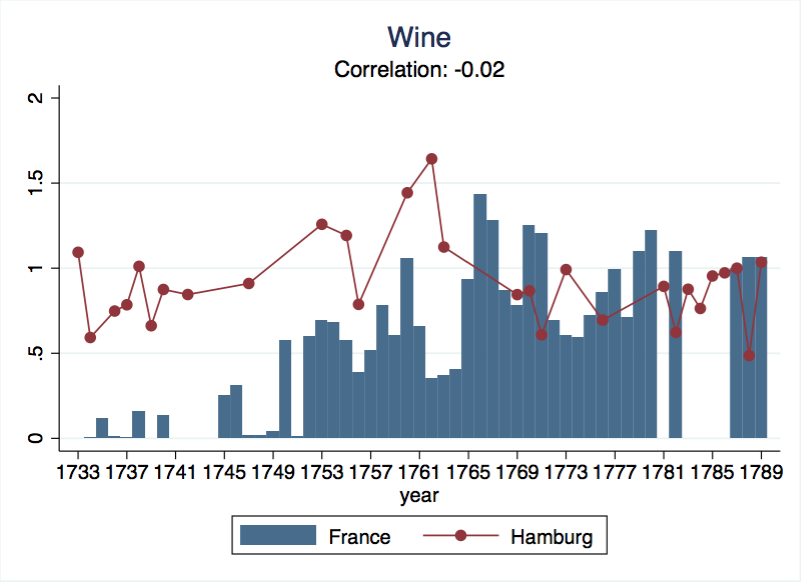
\includegraphics[scale=.28]{wine_long.png}
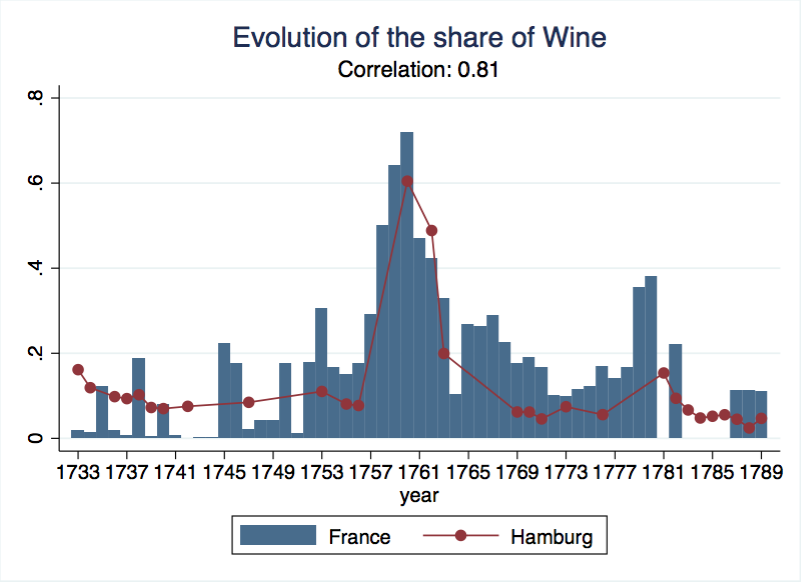
\includegraphics[scale=.28]{wine_share_long.png}
\end{figure}
The evolution of sugar is not too precise comparing the two sources but overall the pattern is quite similar. The fact that strikes the attention is that sugar went to a nearly zero level during Seven Years War (both in share and absolute value) but experienced a less sharp decrease during the American revolutionary war. This pattern is also common to coffee and to a lesser extent to Indigo. On the contrary, in the case of wine and eau de vie, we observe an increase in export, even in absolute value, corresponding to the beginning of the Seven Years War, and then again a decline towards the end of the war. The increase in absolute value lasts till 1761 and then it also collapses together with coffee and sugar, however it remains the major source of export for the war period, especially in terms of share of overall exports. A similar pattern can be noticed during American revolutionary war but on a smaller scale. 


\section{Appendix : Other tables}
\begin{center}
\captionof{table}{Classification Hamburg Large into SITC}
\begin{tabular}{ | l | l | l | l | l | l | }
\hline
	Eau de vie & 1 & Alun & 5 & Vitriol & 5 \\ \hline
	Tobacco & 1 & Cochineal & 5 & Candles & 8 \\ \hline
	Wine & 1 & Gal & 5 & Butter & 0a \\ \hline
	Pernambouc Wood & 2 & Tar & 5 & Fruits & 0a \\ \hline
	Painting Wood & 2 & Indigo & 5 & Rice & 0a \\ \hline
	Cotton & 2 & Minium  & 5 & Vinegar & 0a \\ \hline
	Gum & 2 & Lead Oxyde & 5 & Cacao & 0b \\ \hline
	Lead & 2 & Potassium & 5 & Coffee & 0b \\ \hline
	Saffron & 2 & Soap & 5 & Ginger & 0b \\ \hline
	Spermaceti & 4 & Sumac & 5 & Pepper & 0b \\ \hline
	Olive Oil & 4 & Potassium Bitartre & 5 & Sugar & 0b \\ \hline
	Whale Oil & 4 & Turpentine & 5 & Tea & 0b \\ \hline
	Tallow & 4 & Verdigris & 5 & Iron & 6j \\ \hline
\end{tabular}
\end{center}
\captionof{table}{Table of conversion \textit{Mark Banco}}
\begin{tabular}{ | l | l | l | l | l | l | }
\hline
	1733-35 & 8.3510000000000009 & 1753 & 8.1690000000000005 & 1767 & 7.9130000000000003 \\ \hline
	1736 & 8.19 & 1754 & 8.2230000000000008 & 1768 & 8.2170000000000005 \\ \hline
	1737 & 8.4030000000000005 & 1755 & 8.2490000000000006 & 1769 & 8.2880000000000003 \\ \hline
	1738 & 8.4130000000000003 & 1756 & 8.0129999999999999 & 1770 & 8.4320000000000004 \\ \hline
	1739 & 8.3970000000000002 & 1757 & 7.7830000000000004 & 1771 & 8.4510000000000005 \\ \hline
	1740 & 8.35 & 1758 & 7.6079999999999997 & 1772-74 & 8.4410000000000007 \\ \hline
	1741 & 8.2870000000000008 & 1759 & 7.3840000000000003 & 1775 & 8.4359999999999999 \\ \hline
	1742-46 & 8.2759999999999998 & 1760 & 8.01 & 1776 & 8.4250000000000007 \\ \hline
	1747 & 8.1950000000000003 & 1761 & 8.2959999999999994 & 1777 & 8.4440000000000008 \\ \hline
	1748 & 8.1349999999999998 & 1762 & 8.27 & 1778 & 8.4359999999999999 \\ \hline
	1749 & 8.1890000000000001 & 1763 & 8.24 & 1779-1780 & 8.4250000000000007 \\ \hline
	1750 & 8.35 & 1764 & 8.4700000000000006 & 1781 & 8.4250000000000007 \\ \hline
	1751 & 8.3420000000000005 & 1765 & 8.3689999999999998 & 1783-1798 & 8.4629999999999992 \\ \hline
	1752 & 8.2650000000000006 & 1766 & 7.9950000000000001 & \  & \  \\ \hline
\end{tabular}


\bibliographystyle{plainnat}
\bibliography{bibliography_CSFHT}

\end{document}
